\documentclass{article}
\usepackage{blindtext}
\usepackage{graphicx}

\title{Team 2 Phase 1}
\date{2021 \\ March}

\author{Gabriel L., Jose Lazcano, Jesus Jaime, Yadiel, Fernando, Cristian}

\begin{document}

\maketitle
\section{Name, Place and Date}
ZeitNehmer Workflow Manager\\
Mayaguez, PR\\
March 6, 2021
\section{Introduction}
After various consideration and to streamline the creation of the main feature (workflows) it is important to complete a feature first, which is users accounts. Users accounts can be defined as the user's passport for accesing the features the program offers, these are created by each user and each of them must be unique. This is important because it will be key on features such as:
\begin{enumerate}
  \item Workflow access and assignment.
  \item Roles on workflows
  \item Teams
\end{enumerate}
These are just a rough example of features that require accounts to work at their fullest, more details will be given once they will be worked on.
\vspace{10}

In order for users to access our services they must own an account or create one. With this requirement in mind, the process can be resumed by the following diagram:

\begin{figure}[h!]
    \centering
    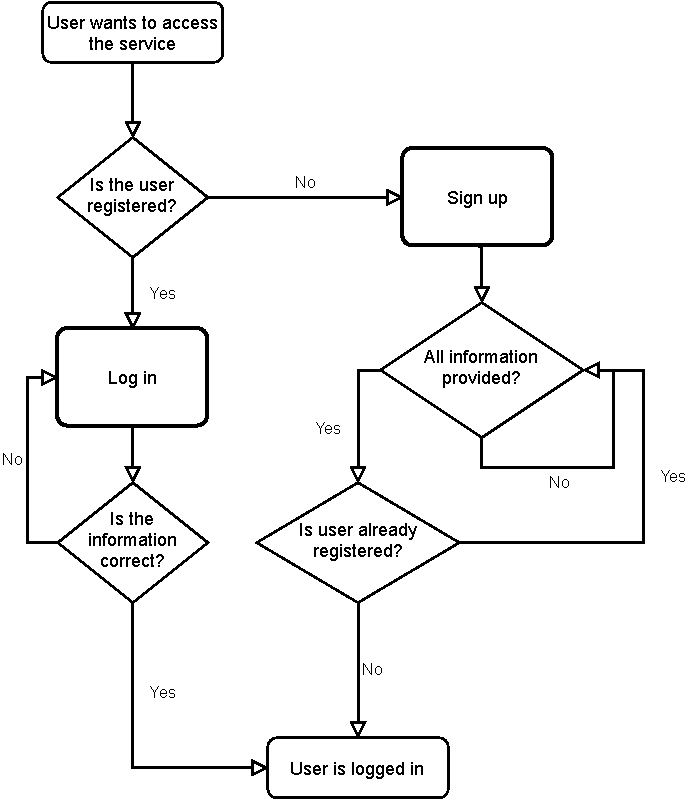
\includegraphics[scale=0.75]{Images/AccessDiagram.pdf}
    \caption{Accesss Diagram}
    \label{fig:figure 1}
\end{figure}

\vspace{110}

To maintain simplicity this process can be divided into different components, these are:

\begin{enumerate}
  \item Sign up
  \item Log in
  \item Users
  \item Registration
\end{enumerate}

There are still components to take in consideration, even though they are not presented explicitly on Figure 1, such as:
\begin{enumerate}
  \item Database
  \item User Interface
\end{enumerate}

As the current state of the platform, some primary pages as been added such as /home, /admin, and /register. These were done using a base.html to reduce code by class inheritance. Since one of the team member is not able to access the class's github all the code can be found here:\\
\url{https://github.com/GaddPetrivoki/ProcrastinatorsRUM}

\section{Sign-Up}
  In order for the user to create an account for now an username and password must be provided, also the password must be confirmed. For the account to be succesfully created the username te user provides must not be the same as any in the database, and the password and password confirmation must match. A sketch as been made that includes:
  \begin{itemize}
    \item A textbox to add the username
    \item A textbox to add a password
    \item A list of some current limitations of the password requirements.
    \item A textbox to confirm the previous password.
  \end{itemize}

  \begin{figure}[h!]
      \centering
      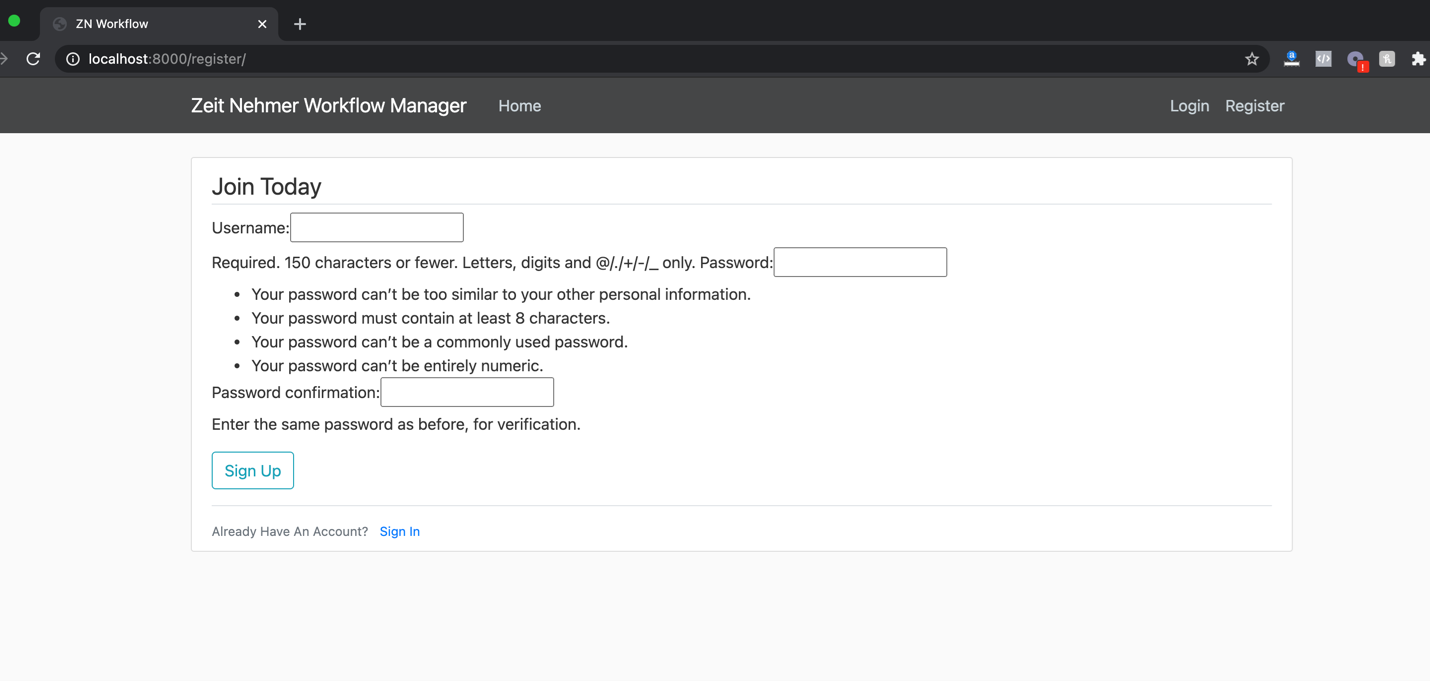
\includegraphics[scale=0.75]{Images/signupMock.png}
      \caption{Sign Up Form Sketch}
      \label{fig:figure 2}
  \end{figure}

\section{Log-In}

  In order for users to access their workflows they will need to log in into their created accounts. This will help keep their workflows secured, since only them and their assigned members will be able to access them.

  \subsection{Implementation}

  Existing users can use their credentials to log into the app, this will be an email or username and a password. The login mechanism uses the users registered with the sign up form to enter the app as an existing user, this is confirmed using the database so that both the email/username and password combination match with the ones registered on the database, if it fails the user will be asked to enter their information again. Once sucessful the user will be able to access all of their content.

  \subsection{User Interface}

  In Figure 3 a prototype of what will be our login page is presented, this includes:
  \begin{enumerate}
    \item A textbox to add the email or username
    \item A textbox to add the user's password
    \item A button to continue with the login
    \item A "Sign up" button in case the user is a new member, this will redirect the user to the sign up procedure discussed before.
  \end{enumerate}

  \begin{figure}[h!]
      \centering
      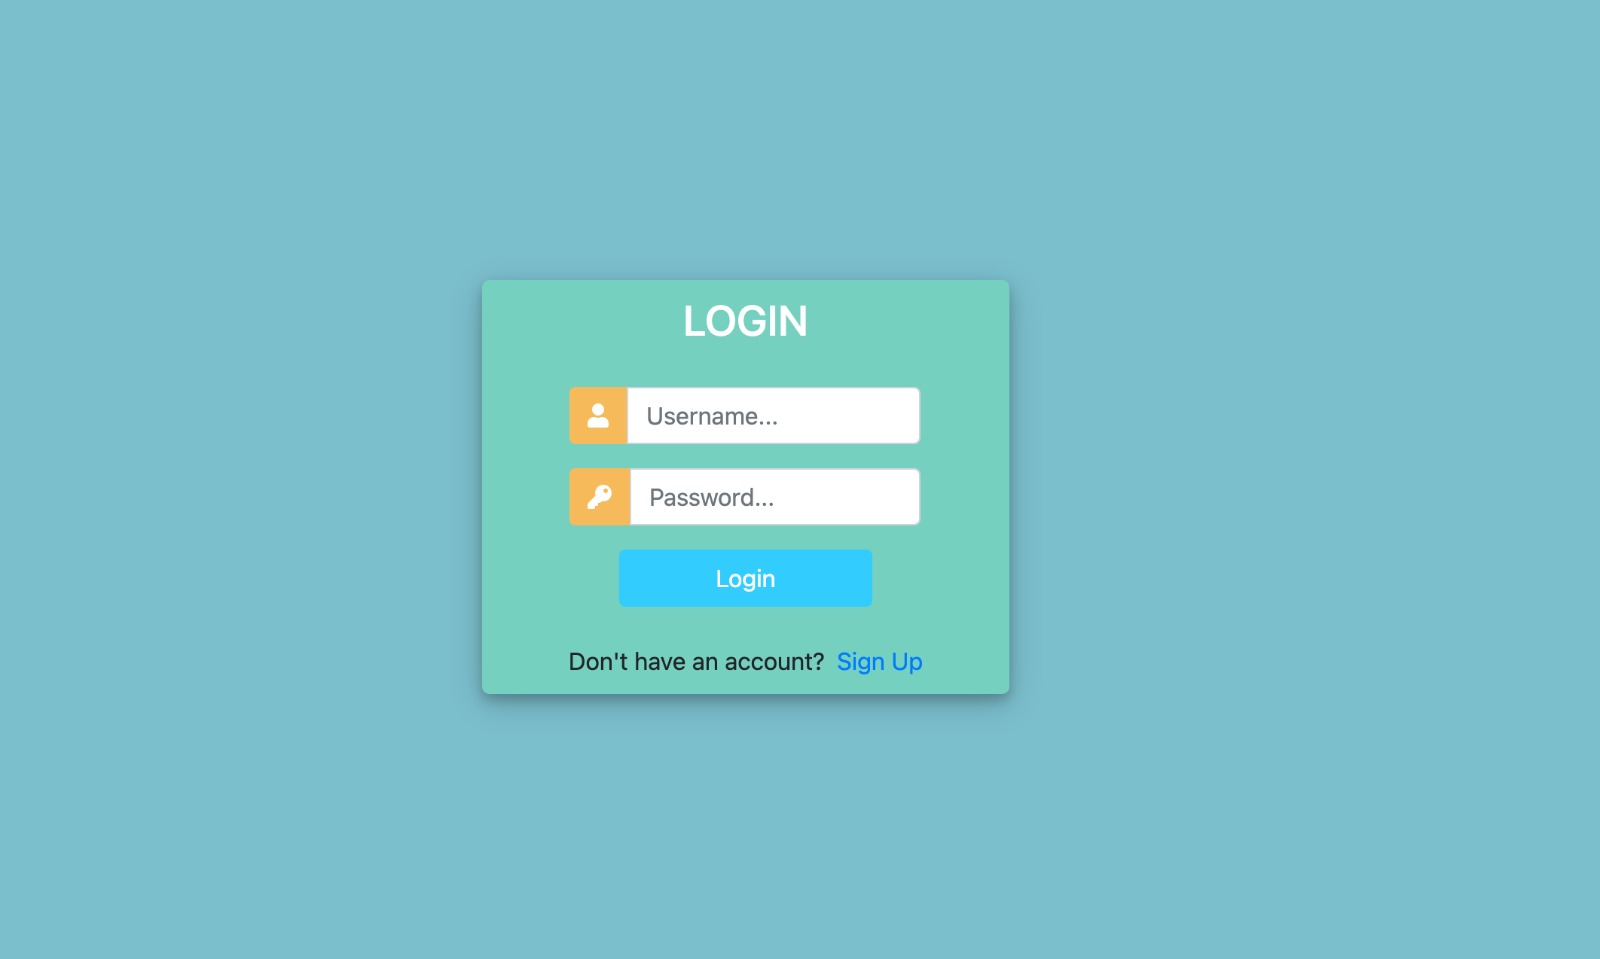
\includegraphics[width=1.2\columnwidth]{Images/loginUI.jpg}
      \caption{Log in Mock-up}
      \label{fig:figure 3}
  \end{figure}

  In order for the user to not lose their account and to minimize that they make another one, a "Forgot password?" button will be added. There an email will be sent to the provided email and a procedure to reset the password will take place. This will be worked on a future sprint.


\section{Users}
  Users can be defined as the people who have made an account and use our platform. There are still some doubts on how this is going to be handle, one of the option is the use of Object Oriented Programming (OOP). These users can be divided intro categories:
  \begin{enumerate}
    \item Administrators
    \begin{quote}
        These users can administrate other users as well as give and take permissions. They will be able to login in a separate from as normal users, like on Figure 4.
        \begin{figure}[h!]
            \centering
            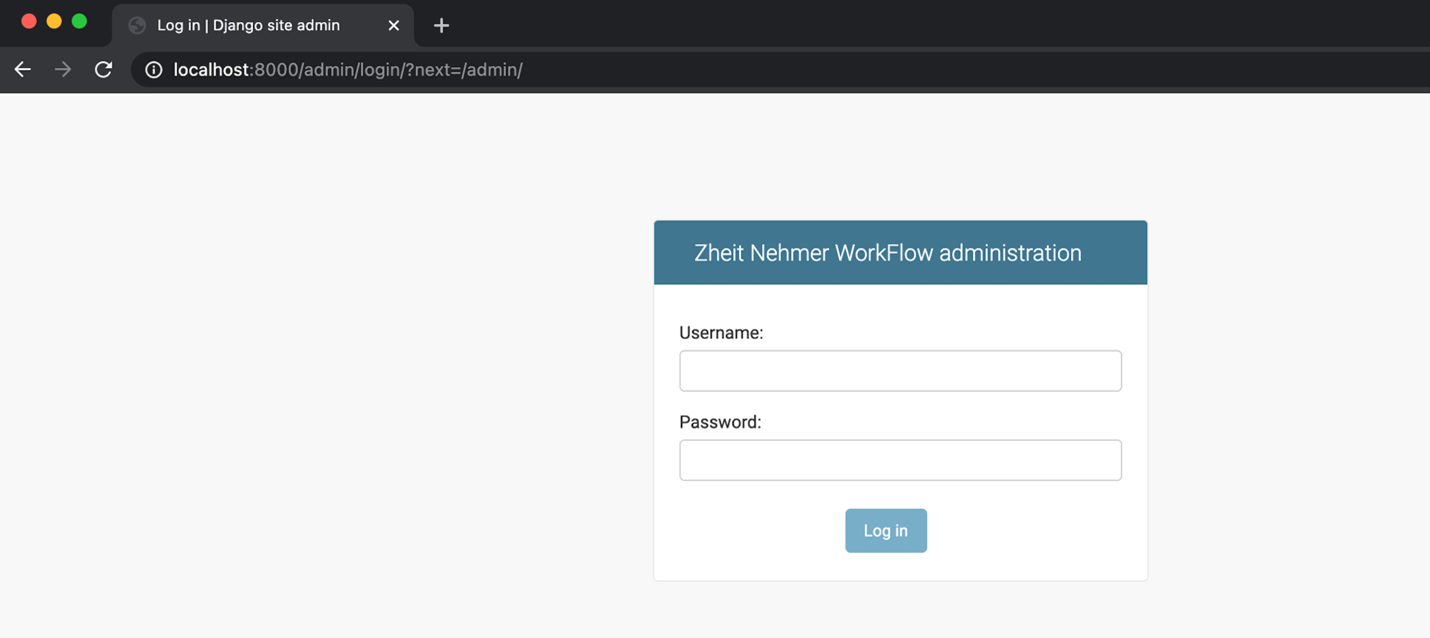
\includegraphics[scale=0.75]{Images/adminLogin.png}
            \caption{Admin Registration}
            \label{fig:figure 4}
        \end{figure}

        \vspace{160}

        This will take the administrator to a management area.

        \begin{figure}[h!]
            \centering
            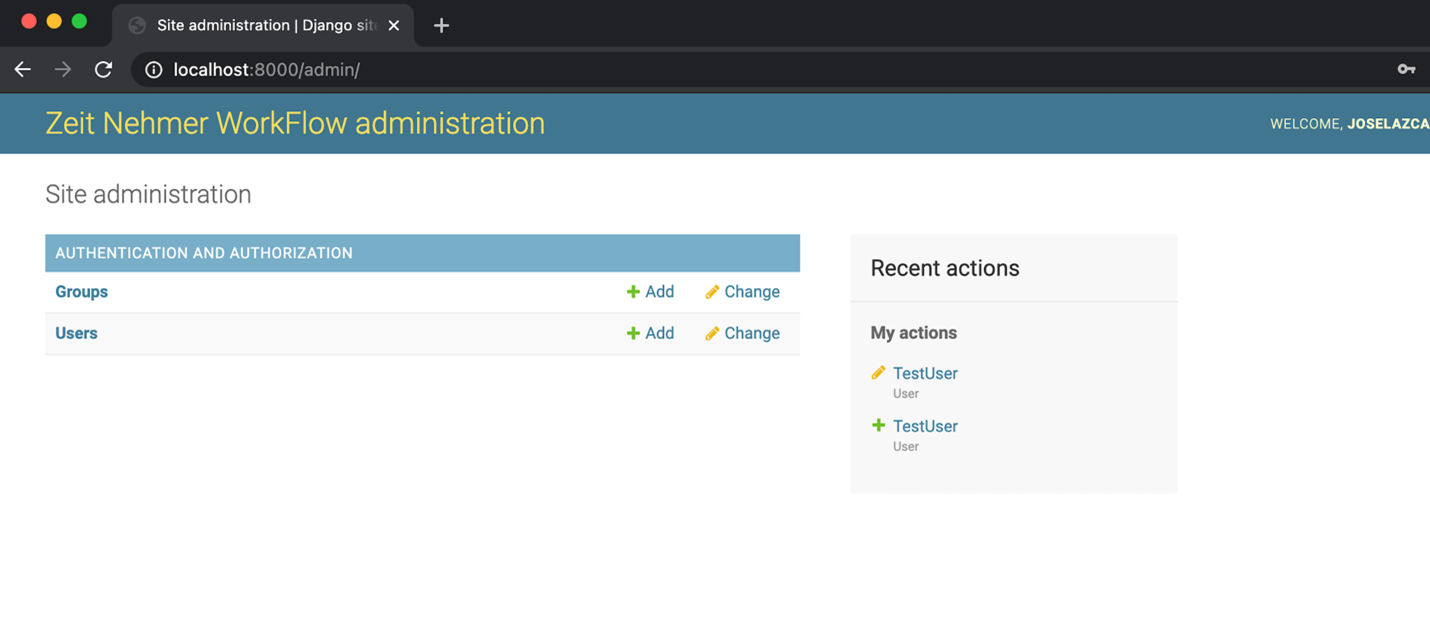
\includegraphics[scale=0.75]{Images/adminManage.png}
            \caption{Administrator Management}
            \label{fig:figure 5}
        \end{figure}



        An administrator can give permissions to users such as:
        \begin{itemize}
          \item Active: decides whether or not the account should have access to the website.
          \item Staff Status: designates whether the user can log into the admin site.
          \item Superuser status: designates that this user has all permissions without assigning them.
        \end{itemize}

        An example of how this permissions will be managed is presented next.

        \begin{figure}[h!]
            \centering
            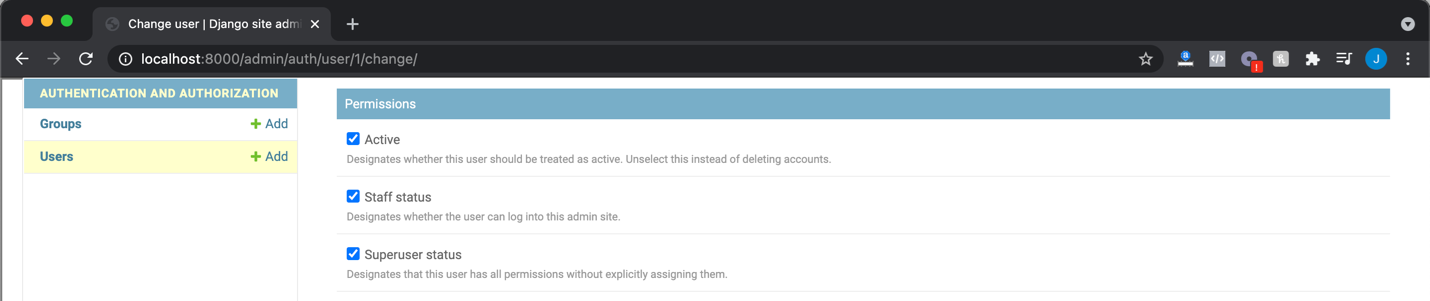
\includegraphics[width=1.2\columnwidth]{Images/adminPerm.png}
            \caption{Administrator Permissions}
            \label{fig:figure 6}
        \end{figure}

        \vspace{100}

        And administrator can also individualy assign or take permissions, such as the next example.

        \begin{figure}[h!]
            \centering
            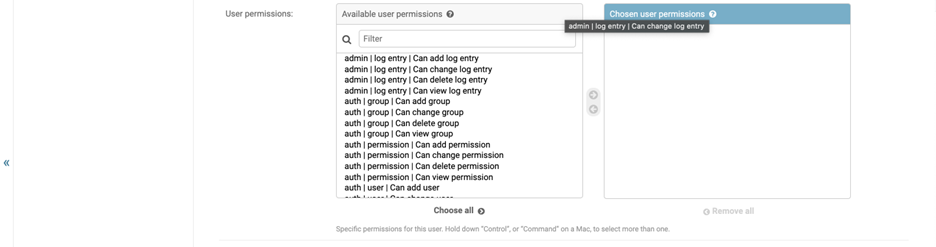
\includegraphics[width=1.2\columnwidth]{Images/adminPerm2.png}
            \caption{Administrator Individual Permissions}
            \label{fig:figure 7}
        \end{figure}
    \end{quote}

    \item Superuser
    \begin{quote}
      A user with all permissions available given.
    \end{quote}

    \item User
    \begin{quote}
      A regular user with the essentials permissions given.
    \end{quote}
  \end{enumerate}

\section{Registration}
The user inputs his data and log in credentials, the system must detect that this is a new account and that information such as email are not already in used by an existing account. If this the case the user will not be able to sign up and will be require to update the information in order to continue. Once succesfull, the system will save the username, password and email into the corresponging user category (Eg. admin, manager or user). There are some elements to take in consideration at the time of registration such as:
\begin{enumerate}
  \item Demographics

  \item Username
  \begin{quote}
    It is important that to no ther user has the same username since this can cause confusion and the server would save two password under the same username.
  \end{quote}

  \item Validation
  \begin{quote}
    The system should verify the user has been able to register without problem and that the username and password combination can be use to access the platform at any time.
  \end{quote}

  \item Password Strength
  \begin{quote}
    The user must be asked to provide a strong password to maintain security at a high level, it must not be the same as the username or any personal information.
  \end{quote}

  \item Group Selection
  \begin{quote}
    If the user has been invited to a group once registered he should be able to accept the invitation and access the group's workflow without problem.
  \end{quote}
\end{enumerate}

\section{Database}
When an account is created the information this contains must be stored remotely and safely. After considering various databases systems, SQL was chosen in order to fulfill this role.
\begin{quote}
  \subsection{What is an SQL Database?}
    SQL is a domain-specific language used in programming and designed for managing data in databases in an organized and efficient way.

\end{quote}

\begin{quote}
  \subsection{Why SQL?}
    In our Software Development Project, we must save, manage, and track data to better execute the features we plan on doing. SQL language can perform best doing this particular task and all future tasks.
\end{quote}

\begin{quote}
  \subsection{Current goals using SQL}
    \begin{itemize}
      \item Link login/registration data to manage POST requests.
      \item Link website to save data on specific databases.
      \item Create or delete database when needed.
      \item Have an SSH or remote connection to it.
      \item Have good security because some databases can contain sensitive data.
    \end{itemize}
\end{quote}

\begin{quote}
  \subsection{Implementation}
    For testing the SQL server we use SQL server 2019 from the Microsoft website and Microsoft SQL Server Management Studio 18.8
    \begin{figure}[h!]
        \centering
        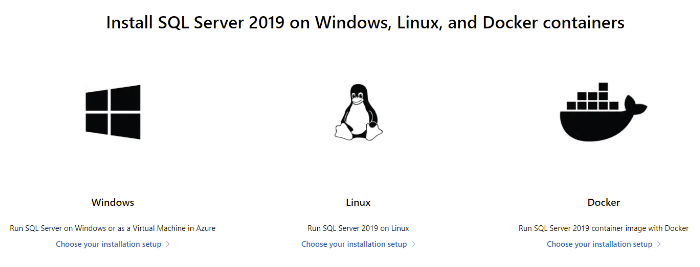
\includegraphics[width=1.2\columnwidth]{Images/sqlServer.png}
        \caption{SQL Server}
        \label{fig:figure 8}
    \end{figure}

    \begin{figure}[h!]
        \centering
        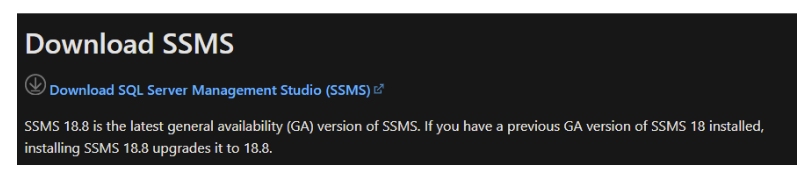
\includegraphics[width=1.2\columnwidth]{Images/ssms.png}
        \caption{SQL Server Management Studio}
        \label{fig:figure 9}
    \end{figure}

    After installing both to a virtual machine we can connecto to our test server in the localhost.

    \begin{figure}[h!]
        \centering
        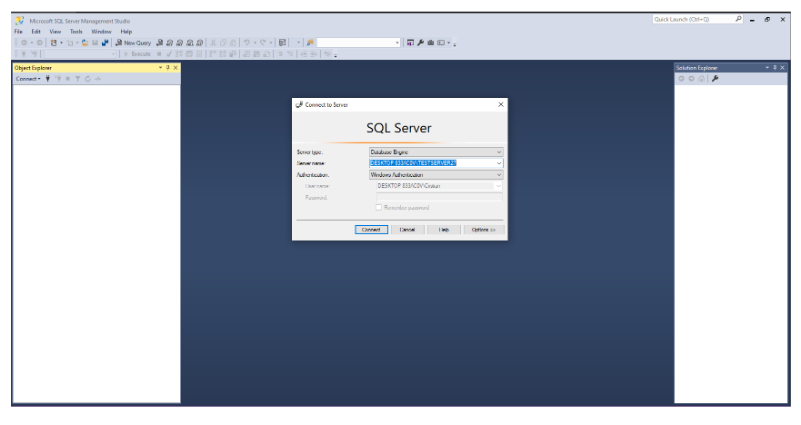
\includegraphics[scale=0.5]{Images/connectingLocalhost.png}
        \caption{Connecting to localhost}
        \label{fig:figure 10}
    \end{figure}

    SQL saves the database with all the data inside tablers and columns, we created a test database and added data to them.
    \begin{itemize}
      \item Database

      \begin{figure}[h!]
          \centering
          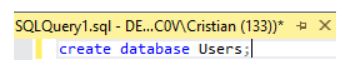
\includegraphics[scale=0.5]{Images/createDatabase.png}
          \caption{Creating Database}
          \label{fig:figure 11}
      \end{figure}


      \item Tables

      \begin{figure}[h!]
          \centering
          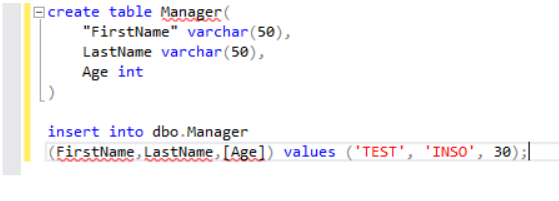
\includegraphics[scale=0.5]{Images/createTables.png}
          \caption{Creating Tables}
          \label{fig:figure 12}
      \end{figure}

      \item Columns
      \begin{figure}[h!]
          \centering
          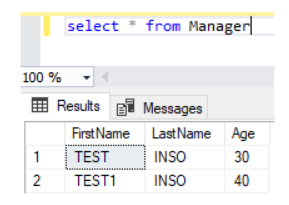
\includegraphics[scale=0.5]{Images/createColumns.png}
          \caption{Creating Columns}
          \label{fig:figure 13}
      \end{figure}

      \vspace{160}

      \item Updating
      \begin{figure}[h!]
          \centering
          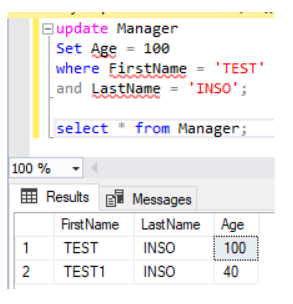
\includegraphics[scale=0.5]{Images/updating.png}
          \caption{Updating Database}
          \label{fig:figure 14}
      \end{figure}

    \end{itemize}

   Adding SQL features to our ptoject can facilitate a lot of data structures in saving, managing, and updating data in just commands. We can hook up SQL utilizing API calls or sending requests to the SQL server.
\end{quote}

\section{Roles}
\vspace{10}
\begin{center}

\begin{tabular}{| l | p{5cm} |}\hline
Name & Main Role \\ \hline
Gabriel L. & fetching information from the data-base\\ \hline
Yadiel     & Back-End\\ \hline
Cristian   & Front-end-design \\ \hline
Fernando   & Back-End \\ \hline
Jesus	   & Information storage\\ \hline
Jose Lazcano  & User Interface \\ \hline
\end{tabular}

\end{center}
\end{document}
